\documentclass[10pt,a4paper]{article}

% Standard required packages
\usepackage[utf8]{inputenc}
\usepackage{amsmath,bm}
\usepackage{graphicx}
\usepackage{caption}
\usepackage{subcaption}
\usepackage{hyperref}
\usepackage{systeme}
\usepackage{mathbbol}
\usepackage{mathtools}
\usepackage{listings}
\hypersetup{
    colorlinks,
    citecolor=black,
    filecolor=black,
    linkcolor=black,
    urlcolor=black
}
\graphicspath{ {../images/} }

\begin{document}

\begin{titlepage}
    \begin{center}
        \vspace*{1cm}
        \Huge\textbf{Assignment 3}\\
        \vspace{1.5cm}
        \Large Author:
        \textbf{Paolo Renzi}\\
        \Large Contributors:\textbf{Bruno Francesco Nocera 1863075, Silverio Manganaro 1817504, Simone Tozzi, 1615930, Leonardo Colosi 1799057, Jacopo Tedeschi 1882789, Amine Ahardane 2050689.}
        \vspace{0.5cm}
        \vfill
        
\includegraphics[width=0.7\textwidth]{../images/sapienza_logo.png}
        \vfill
        \vspace{0.8cm}
        \Large \textit{MARR, RL}\\
        \today
    \end{center}
\end{titlepage}
\newpage

\section*{Theory}
\subsection*{Problem 1}
The environmenthas 2 actions and a 2 dimensionsional state space. the policy and action-state value function approximators are the following:
\begin{equation*}
    \pi_\theta (a=1|s) = \sigma(\theta^T x(s)) = \frac{1}{1+e^{-(\theta^T x(s))}}
\end{equation*}
\begin{equation*}
    Q_\omega(s,a=0) = \omega_0^T x(s)
\end{equation*}
\begin{equation*}
    Q_\omega(s,a=1) = \omega_1^T x(s)
\end{equation*}
While the transition function is this:
\begin{equation*}
    x(s0) = (1, 0)^T , a_0 = 0, r_1 = 0, x(s1) = (0, 1)^T , a_1 = 1
\end{equation*}

To update the weights of the networks we follow the Actor-Critic algorithm:
\begin{itemize}
    \item Compute the state from the approximation function
    \item Compute the TD error
    \item Pick the Critic weights to minimize the TD error 
    \item Update the Actor weights' in the same direction 
\end{itemize}

So the approximated state is:
\begin{equation*}
    Q_w(s, a = 0) = w_0^Tx(s) = \begin{pmatrix} 0.8 & 1 \end{pmatrix} \begin{pmatrix} 1 \\ 0 \end{pmatrix} = 0.8
\end{equation*}

\begin{equation*}
    Q_w(s, a = 1) = w_1^Tx(s) = \begin{pmatrix} 0.4 & 0 \end{pmatrix} \begin{pmatrix} 1 \\ 0 \end{pmatrix} = 0
\end{equation*}

With this we can compute the TD error

\begin{equation*}
    \delta = 0 + 0.9*(0) - 0.8 = -0.8
\end{equation*}

To pick the appropriate weights of the Critic we use gradient descent  

\begin{equation*}
w_0 = w_0 + \alpha\gamma \nabla_w Q_{w_0} (x(s_0), a_0) = \begin{pmatrix} 0.8 & 1 \end{pmatrix} -0.8 * 0.1 \begin{pmatrix} 1 \\ 0 \end{pmatrix} = \begin{pmatrix} 0.72 & 1 \end{pmatrix}
\end{equation*}

To update the Actor weights' we can use gradient descent again but it would be not 0 only if the action $a_1 = 0 $was taken at state$ x(s_0) $we would not use the gradient of$ Q(x(s), a1) $for the update in this step. Using
instead the gradient of $Q(x(s), a0) $lead to no change for the vector $w_1$

\begin{equation*}
    w_1 = w_1 + \alpha\gamma \nabla_w Q_{w_1} (x(s), a_0) = \begin{pmatrix} 0.4 & 0 \end{pmatrix} -0.8 * 0.1 \begin{pmatrix} 0 \\ 0 \end{pmatrix} = \begin{pmatrix} 0.4 & 0 \end{pmatrix}
\end{equation*}

There is a variation of the Actor-Critic algorithm that updates both $w_0$ and $w_1$ using the respective gradients even if one of the associated actions was not taken, as part of an off-policy learning method, so we would update the weights like this

\begin{equation*}
    w_1 = w_1 + \alpha\gamma \nabla_w Q_{w_1} (x(s_1), a_1) = \begin{pmatrix} 0.4 & 0 \end{pmatrix} -0.8 * 0.1 \begin{pmatrix} 0 \\ 1 \end{pmatrix} = \begin{pmatrix} 0.4 & -0.08 \end{pmatrix}
\end{equation*}

Finally we can compute the new value of $\theta$ according to:

\begin{equation*}
    \theta = \theta + \alpha\delta\nabla_\theta log \pi_\theta (a|s)
\end{equation*}

To calculate the gradient we need the value of $ \pi_\theta (a = 0|s) $. To obtain this expression we could make the observation that, since
the action space is binary and $\pi$ represent a probability distribution over actions,
$\pi_\theta (a = 0|s) = 1 - \pi_\theta (a = 1|s)$. After established this we can proceed with the
computation of the gradient:

$\pi_\theta (a = 0|s) = 1 - \pi_\theta (a = 1|s)$
\begin{equation*}
    \nabla_\theta log(1 - \pi_\theta (a = 1|x(s_0))) =
\end{equation*}
\begin{equation*}
    \nabla_\theta log ( 1 - \frac{1}{1 + e^y} ) = \nabla_\theta log ( \frac{1 + e^{y - 1}}{1 + e^y} ) 
\end{equation*}

With $y = -(\theta_T x(s)) $

\begin{equation*}
    \nabla_\theta log ( \frac{e^y}{1 + e^y} ) =  \nabla_\theta log(e^y) - \nabla_\theta log ( \frac{e^y}{1 + e^y} ) = 
\end{equation*}

\begin{equation*}
    \nabla_\theta y - \nabla_\theta log(1 + e^y )
\end{equation*}
substituting y
\begin{equation*}
    -x(s) + \frac{x(s) * e^{-(\theta_T x(s))}}{1+e^{-(\theta_T x(s))}}
\end{equation*}
and taking the gradient.
\begin{equation*}
    \frac{-x(s) - x(s) * e^{-(\theta_T x(s))} + x(s) * e^{-(\theta_T x(s))} }{1+ e^{-(\theta_T x(s))}}
\end{equation*}
Evaluating in $x(s_0), \theta_0$
\begin{equation*}
    -x(s_1) + e^{-(\theta_T x(s))} = -\begin{pmatrix} 0.73 // 0 \end{pmatrix}
\end{equation*}
To obtain the final evaluation we should take in account that:
\begin{equation*}
    \theta_T x(s) = 1
\end{equation*}
\begin{equation*}
    1 + e^{-1} = 1.36
\end{equation*}
\begin{equation*}
    \frac{1}{1+e^{-1}} = 0.73
\end{equation*}
The final value for $\theta$ is given by:

\begin{equation*}
    \theta = \theta_0 + \alpha \ \nabla_\theta log \pi_\theta (a = 0|x(s_0)) = \begin{pmatrix} 1 & 0.5 \end{pmatrix} +0.8 * 0.1 *\begin{pmatrix} 0.73 \\ 0 \end{pmatrix} = \begin{pmatrix} 1.05 & 0.5 \end{pmatrix}
\end{equation*}






\newpage
\section*{Code}

\subsection*{World models}
To complete the car racing environment from the gymnasium library, it is a simplified version of a 2d racing game with UI on screen, with inputs that can be either continuous or discrete.  The reward is
-0.1 every frame and +1000/N for every track tile visited, where N is the total number of tiles visited in the track. This means that the reward is skewed more towards having the car go rather than having it go on track beacause 
the reward is the same whether it stays still or moves when it's outside of the track.
I tried to solve the discrete version in particular, to do so i implemented the world Models solution as proposed in \href{https://doi.org/10.5281/zenodo.1207631}{this paper},
in particular the version without the RNN-MDN. This model is composed of two parts a Variational AutoEncoder (VAE) and a linear layer.


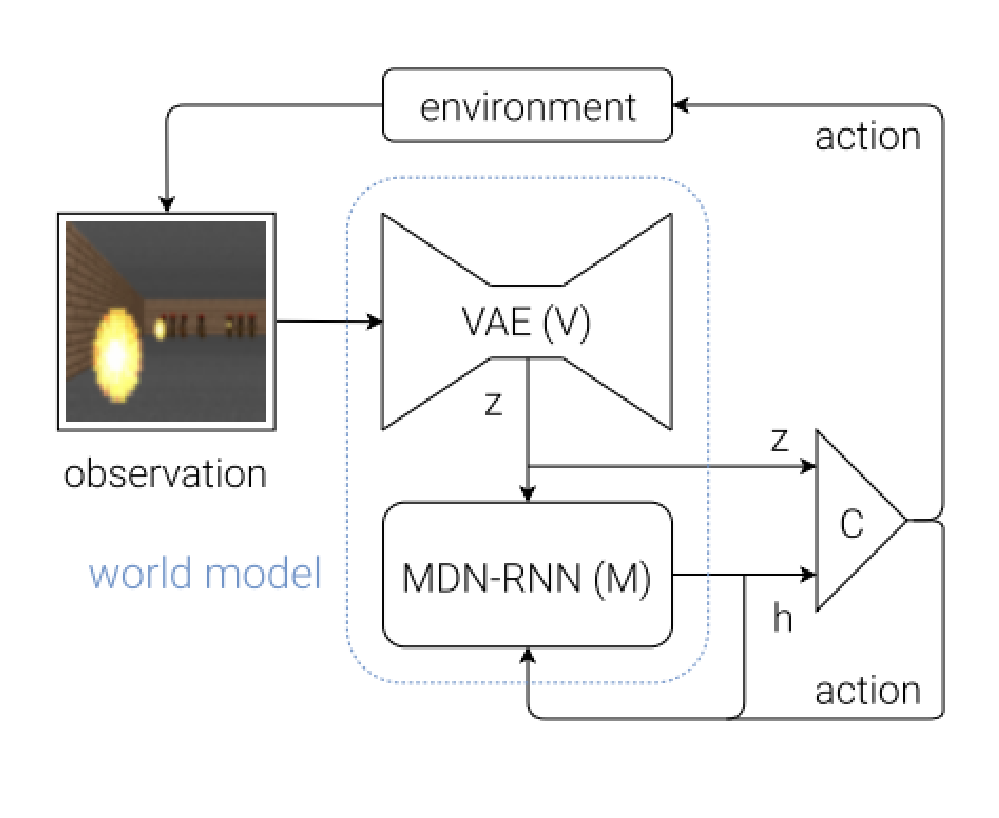
\includegraphics[scale=0.4]{model.png}

The VAE I implemented is composed of 3 convoultional layers with RELU as activation function, an average pooling layer, and a final linear layer as encoder, and only transposed convolutions layers for the decoder with RELU for all the layers except the last that uses a sigmoid.
The VAE also has two linear layers that derives the mu and the logvar from the latent space, that is a vector of dimension 32. The dataset for the VAE is created by doing a random rollout and selected with this code:
\begin{lstlisting}
a = int(np.random.rand()*3 +1).
\end{lstlisting}
I also divided the learning in 4 parts with a decresing learning rate, from 2.5e-3 to 1e-7, with a batch size of 128 and Kullback-Leibler Divergence (KDL) together with Binary Cross Entropy With Logits Loss.

\begin{equation*}
    KLD = -\frac{1}{2} * \sum_{j = 1}^{J} (1 + log((\sigma j )^2) - (\mu_j )^2 - (1\sigma_j )^2) 
\end{equation*}

\begin{equation*}
    BCE = \frac{1}{n} * \sum_{j = 1}^{N} (y^i log(\hat{y^i}) + (1 - y^i) log(1 - \hat{y}i))
\end{equation*}

With this results for the reconstruction of the images

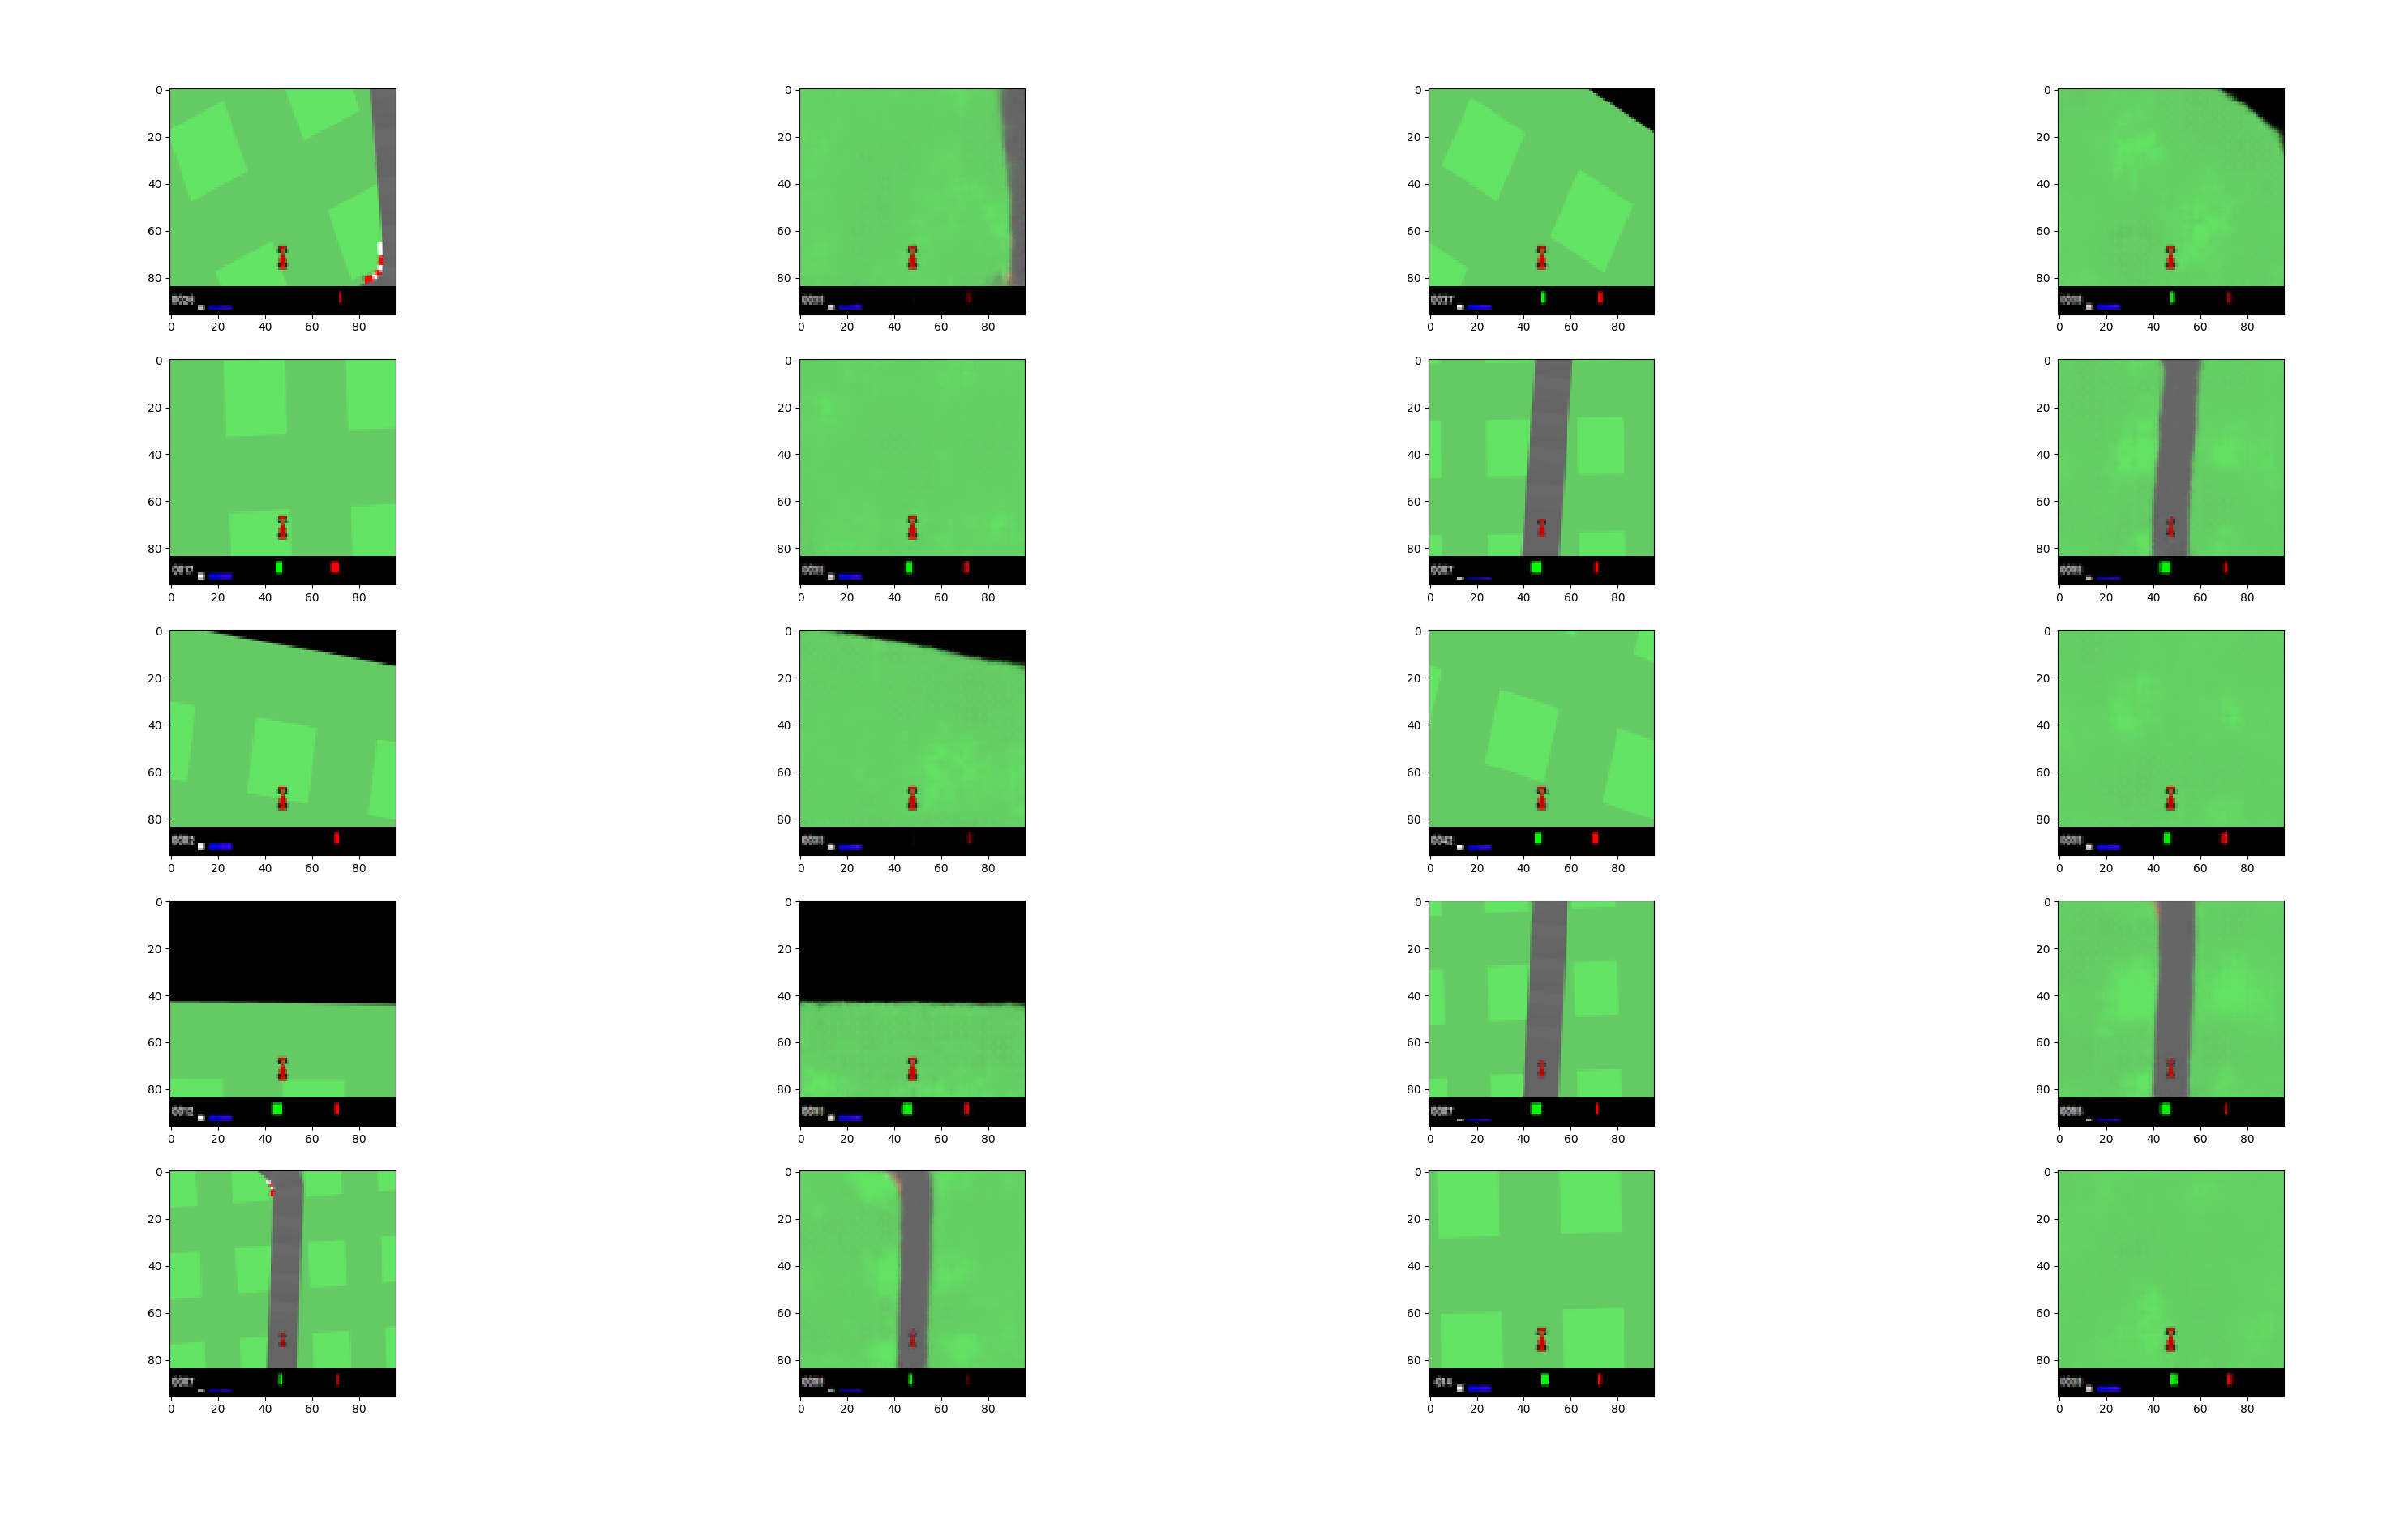
\includegraphics[scale=0.14]{VAEres.png}

To train the linear layer first of all i check if I have saved a model i already trained to initialize the training, then I used the Covariance Matrix Adaptation Evolution Strategy (CMA-ES). 
To evaluate the solutions i run them on the environment and sum the cumulative reward to a "temperature" value of 1000.
To have this policy act first it encodes the state to get the latent space vector (after making sure it has the right dimensions and order of dimensions) that then gets passed to the linear layer to have it output the action probabilities that is used to select the action using argmax






\newpage

\begin{thebibliography}{9}
    \bibitem{article}

    \emph{World Models} by \textit{Ha, David and Schmidhuber, Jürgen},  link: https://doi.org/10.5281/zenodo.1207631, doi 10.5281/ZENODO.1207631, publisher Zenodo, year 2018, copyright Creative Commons Attribution 4.0
    
\end{thebibliography}

\end{document}